

\documentclass[a4paper,10pt]{article}
\usepackage{listings,color,epsfig,amsmath,url}
\definecolor{codecolor}{rgb}{0.99,0.97,0.94} % color values Red, Green, Blue
\definecolor{commentcolor}{rgb}{0.1,0.5,0.1} % color values Red, Green, Blue
\definecolor{stringcolor}{rgb}{0.3,0.1,0.1} % color values Red, Green, Blue
\newcommand{\Code}[1]{\texttt{#1} }
\newcommand{\code}[1]{\Code{#1} }
\newcommand{\DB}   {\code{{MOOSDB}}}
\newcommand{\MA}   {\code{{MOOSApp}}}
\newcommand{\Ignore}[1]   {}




\lstset{ frame = shadowbox,
 %language=[Visual]{c++},
 rulesepcolor=\color{black},
 basicstyle=\small } \lstset{
backgroundcolor=\color{codecolor},
keywordstyle=\color{blue}\bfseries,
commentstyle=\color{commentcolor},
stringstyle=\color{stringcolor}\ttfamily, linewidth =
1.2\linewidth,
breaklines=true} %

\lstset{language=C++}


% Title Page
\title{Bridging Communities with \code{pMOOSBridge}}
\author{Paul Newman}



\begin{document}
\maketitle

\begin{center}

\epsfig{file=images/moose6.eps,width = 0.2\linewidth}
\end{center}
\begin{abstract}
This document will give you a description of how to use \code{pMOOSBridge} to link multiple MOOS communities together.
\end{abstract}


\tableofcontents

\section{Introduction}

\code{pMOOSBridge} is a powerful tool in building MOOS-derived
systems. It allows messages to pass between communities and is
able to rename the messages as they are shuffled between
communities. Many of the sections in this document rely on
\code{pMOOSBridge} to set up different communications topologies. There is no correct topology --- choose one that
works for your own needs.
\begin{figure}[ht]
\centering 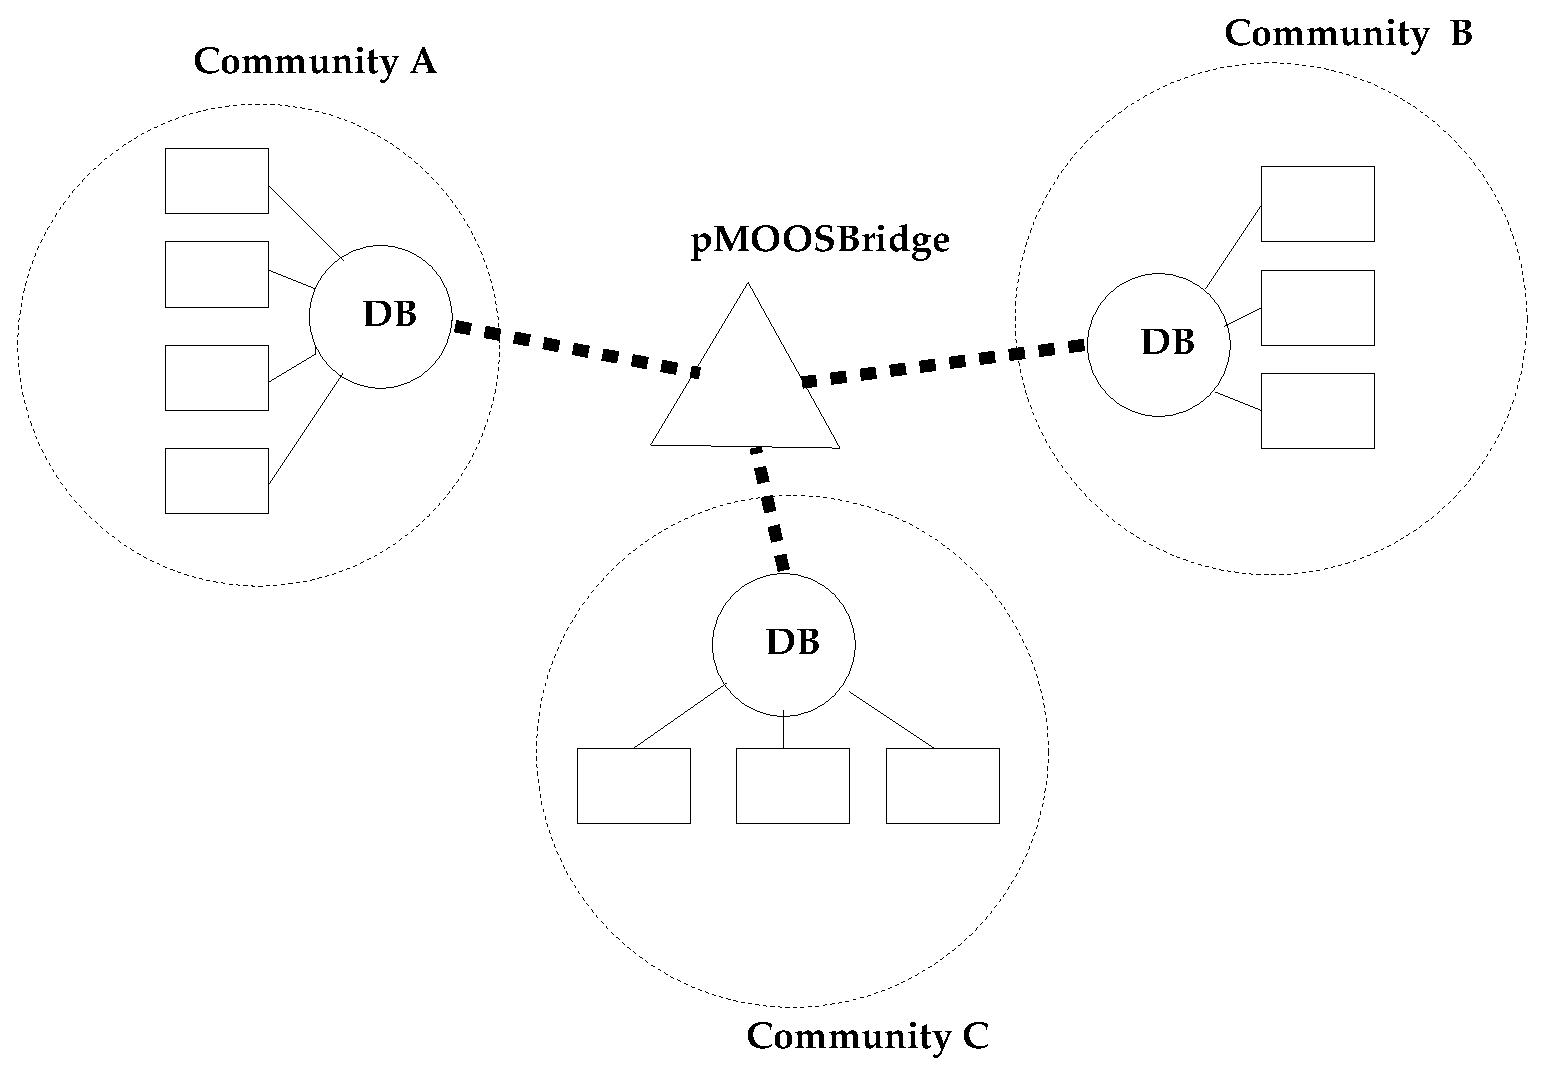
\epsfig{file = images/pMOOSBridge.eps , width = 0.6\linewidth}
\caption{A possible MOOSBridge
configuration. One instance of \code{pMOOSBridge} can ``talk'' to a limitless
number of communities. The configuration block specifies what
should be mapped or ``shared'' between communities and how it
should be done. The \code{SHARE} command specifies precisely what
variables should be shared between which communities.}\label{fig:MOOSBridge1}
\end{figure}
One instance of \code{pMOOSBridge} can ``talk'' to a limitless
number of communities. 

\section{Basic Configuration}
The configuration block specifies what
should be mapped or ``shared'' between communities and how it
should be done. The \code{SHARE} command specifies precisely what
variables should be shared between which communities and the
syntax is intuitive:\\

\code{SHARE= {\it{Comm@Host:Port[V1[,V2...]] $->$ Comm@Host:port
[V1,V2...]}}}\\

The triplet Comm@Host:Port is a description of a community ---  name and hostname/port pair. The community
description can be omitted on the LHS of the arrow, in which case the mission-file-scope defaults are assumed (see the example below).
Each variable (``V'') on the LHS (source) community will be inserted into the community on the RHS
If no variable names are specified on the RHS (destination) community the original names are used, otherwise
there is a one-to-one mapping between variable names on the LHS and new variable names (aliases) on the RHS. If however
there are more named shared variables than aliases, the variables for which an alias is not specified retain their original names. For example
\begin{verbatim}
SHARE= VehA@nym.robots.ox.ac.uk:9000 [GPS_X]->VehB@kayak.mit.edu:9000 [GPS_X]
\end{verbatim}
Here the variable \code{GPS\_X} is shared between a community called ``VehA'', running from a \DB on the machine called
``nym.robots.ox.ac.uk'' listening on port 9000, is being inserted into a community called ``VehB'' using a \DB running on the machine called
``VehB@kayak.mit.edu'' also listening on port 9000. In both communities the variable is called ``GPS\_X''. However when viewed with
something like \code{uMS} (see the document on Graphical Tools) it can be seen that the \code{m\_sOrginatingCommunity} member of the \code{MOOSMsg}
carrying this data in the ``VehB'' commmunity will be ``VehA''.

\begin{verbatim}
SHARE= VehA@nym.robots.ox.ac.uk:9000 [GPS_X]->VehB@kayak.mit.edu:9000 [GPS_X_A]
\end{verbatim}
This is similar to the above example, only \code{pMOOSBridge} will rename ``GPS\_X'' to ``GPS\_X\_A'' in the
destination community. The next example shows how the source address need not be specified. When omitted the source community is
taken to be the community on which \code{pMOOSBridge} is running at the time. This example also shows how destination variable names may be omitted, in
which case the original (source community) variable name is preserved.
\begin{verbatim}
SHARE= [GPS_X]->VehB@kayak.mit.edu:9000
\end{verbatim}
Finally, more than one mapping can be specified in one line:
\begin{verbatim}
SHARE= [GPS_X,OVEN_TEMP]->VehB@kayak.mit.edu:9000 [GPS_X_A]
\end{verbatim}
Here GPS\_X is being mapped and renamed to \code{GPS\_X\_A} in community ``VehB'' but the variable \code{OVEN\_TEMP} is simply being shared without renaming.
It is important to realise that sharing is not bidirectional. In this case, a process notifying change in \code{GPS\_X\_A} in community ``VehB'' \emph{would not}
result in pMOOSBridge notifying the \DB in community ``VehA'' that ``GPS\_X'' has changed.



\subsection{Specifying Sharing Bandwidth}

Recall  that when using the \code{CMOOSCommClient} class or \code{CMOOSApp::Register()}  it is possible to specify the maximum rate at which one wishes to be notified of variable changes. So for example if a variable is actually been changed at 50Hz it is possible to request a notification at no more that 1Hz. Alternatively one can register to receive every notification. The same paradigm exists in code \code{pMOOSBridge} although it cannot be configured on a per variable basis. By setting \code{BridgeFrequency} to be some integer value the maximum frequency of notifications being bridge between communities can be controlled. For example
\begin{center}
\code{BridgeFrequency} = 10
\end{center}
will mean that no variables are bridge with frequency greater than 10Hz. A special case is
\begin{center}
\code{BridgeFrequency} = 0
\end{center}
which means that {\textbf{every}} change in bridged variables is sent to destination communities.


\section{Topologies}
The configuration of \code{pMOOSBridge} facilitates many connection topologies. One such topology is show in Figure \label{fig:MOOSBridge1}, here we have one central \code{pMOOSBridge} joining  several communities together. A common alternative is shown in \label{fig:MOOSBridge2} in which each community has its own bridge. Although functionally the two setup are identical the latter offers the opportunity to use UDP sharing as discussed in Section  \ref{Sec:UDP}.

\begin{figure}[ht]
\centering 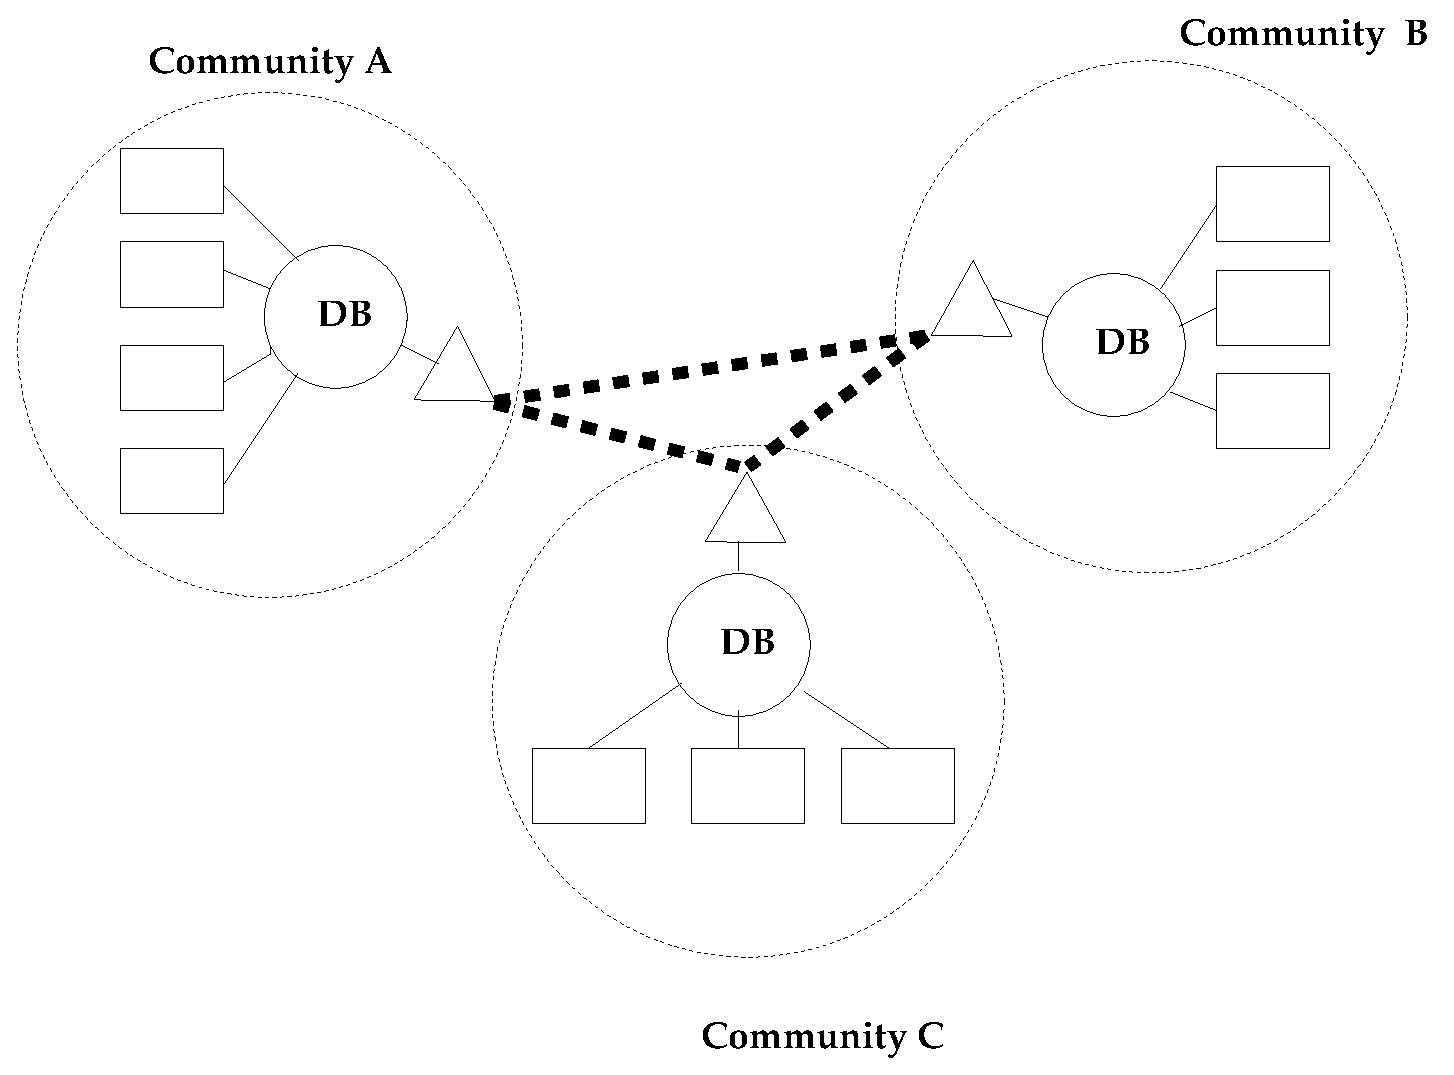
\epsfig{file = images/pMOOSBridge2.eps , width =
0.6\linewidth} \caption{An alternative MOOSBridge Configuration
--- one bridge per community. This may be preferable; it is undesirable to have one process manage all
the sharing of data. However it offers no \emph{functional} advantage over the topology shown in Figure
\ref{fig:MOOSBridge1}. That said, this is the only configuration in which UDP sharing can be used --- see section \ref{:Sec:UDPSharing}}\label{fig:MOOSBridge2}
\end{figure}



\section{Sharing by UDP}\label{Sec:UDP}

It is possible that an application domain requires that the link between distinct MOOS communities by made not with tcp/ip but with udp. An obvious example would be when intermittent wireless communications is available between 
communities  - using tcp/ip here (the protocol used by standard MOOS comms) will result in poor performance as it is connection oriented substantial time will be expended behind the scenes in reconnecting and blocking read and write calls at various places in the comms architecture \footnote{when a write completes on a tcp/ip socket you are guaranteed that the data has arrived at its destination}. UDP however offers more of a ``fire and forget'' paradigm - if packets can make it across the inter-community link then they will but the sender is oblivious to their fate.

\subsection{Basic Configuration}
Before describing how UDP sharing can be configured it is important to note the following points.
\begin{itemize}
\item  UDP sharing is only possible when using the topology shown in Figure \ref{fig:MOOSBridge2} --- that is with one \code{pMOOSBridge} running in each community.
\item Any bridge that wants to receive transmissions from other bridges (think ``bridge= community' because of the above point --- one bridge per community for UDP sharing) must be told the port on which it is to listen for incoming UDP packets. This is done with the \code{UDPListen} variable in the configuration block.  For example 
\begin{center}
\code{UDPListen} = \code{9100}
\end{center}
will cause the Bridge to listen on port 9100.
\item \code{pMOOSBridge} supports to modes of UDP sharing. The first called ``Directed Sharing'' sends MOOS mail to just one named recipient (another Bridge in another community) . The second mode, called ``Broadcast Sharing''  sends data to all and sundry  - any bridge who is listening on the relevant port will receive the transmission.
\item Both UDP sharing modes are configured with the \code{UDPShare} keyword.
 \end{itemize}
 
 
\subsection{UDP Directed Sharing}

In this case the syntax is similar to the regular \code{SHARE} already discussed although the source community need not be described because the enforced topology constraint means this is implicit. For example, for  a Bridge running on community ``VehA'' a line such as this
\begin{verbatim}
UDPSHARE= [GPS_X]->VehB@kayak.mit.edu:9200 [GPS_X_VEH_A]
\end{verbatim}

in the pMOOSBridge configuration block will cause the \code{GPS\_X} variable within community ``VehA'' to be sent to a \code{pMOOSBridge} running on Community ``VehB'' which has been configured to listening for incoming UDP packets on port 9200 on a machine called kayak.mit.edu. This data will appear as \code{GPS\_X\_VEH\_A} in the ``VehB'' community.


\subsection{UDP Broadcast Sharing}

It is also possible to broadcast messages across the network indiscriminately meaning that every pMOOSBridge listening on the required port will receive the MOOS variable and insert it inot its local community's  \code{MOOSDB}. The required syntax is exactly as for the directed UDP share, the difference comes from specifying the destination address to be ``all@broadcast'' followed by the required port address. So, carrying on with the example above,
\begin{verbatim}
UDPSHARE= [GPS_X]->all@broadcast:9200 [GPS_X_VEH_A]
\end{verbatim}
will mean any \code{pMOOSbridge} listening on port 9200 on the local network will receive \code{GPS\_X\_VEH\_A}  which was originally  \code{GPS\_X}  in community ``VehA'' (assuming of course that the bridge configured with this line is still runing in a community called ``VehA'').
 



\subsection{Example Configurations}



\lstinputlisting[basicstyle=\footnotesize, caption = {pMOOSBridge configuration block for a community called V1 illustrating two types of UDP sharing ---directed and broadcast },label = {Example:V2}
]{examples/V1.moos}

\lstinputlisting[basicstyle=\footnotesize, caption = {pMOOSBridge configuration block for a community called V2 publishing  one variable via directed UDP sharing and one via regular tcp/ip},label = {Example:V2}
]{examples/V2.moos}





\end{document} 